
% Introduzione +++++++++++++++++++++++++++++++++++++++++++++++++++++++++++++++++

Le equazioni che descrivono i fenomeni fisici hanno carattere tensoriale,
 cioè sono indipendenti dal sistema di coordinate nelle quali vengono scritte.
\'E importante capire la natura tensoriale delle leggi fisiche, capirne
 l'\textit{invarianza} rispetto ai sistemi di coordinate ed essere in grado di
 scrivere correttamente le equazioni nei sistemi di coordinate più vantaggiosi
 per la descrizione del fenomeno fisico e per la soluzione dei problemi.

\vspace{0.2cm}
In questo capitolo verrà usata la notazione di Einstein: è sottointesa la sommatoria
 sugli indici ripetuti in una espressione. Per chiarezza,
\begin{equation}
 a_k b_k = \displaystyle\sum_k a_k b_k .
\end{equation}

Si considerano qui \textbf{solo spazi vettoriali dotati di 
 prodotto interno}, per i quali è possibile evitare di introdurre concetti
 più generali, ma più astratti e del tutto inessenziali per una prima
 introduzione ai tensori e al calcolo tensoriale: ad esempio è possibile
 ``schivare'' le definizioni di spazio e base duale (parente di quella che qui
 verrà chiamata \textit{base reciproca}), isomorfismi e altri concetti più
 ``matematici''. Vengono comunque dati alcuni riferimenti per una trattazione esaustiva
 dell'argomento. 

% Prime definizioni ++++++++++++++++++++++++++++++++++++++++++++++++++++++++++++
\section{Richiami di algebra lineare}

% Base e Componenti contravarianti ----------------
\begin{definition}[Componenti contravarianti]
Sia $\mathcal{V}$ uno spazio vettoriale, sia $\bm{v}$ un elemento di $\mathcal{V}$
 e $\{ \bm{b}_k \}_{k=1:N}$ una base\footnote{Una base è un insieme minimale di vettori linearmente indipendenti. La dimensione dello spazio vettoriale coincide con il numero di elementi di una sua base.} di $\mathcal{V}$; si può scrivere il vettore $\bm{v}$ in componenti rispetto alla base $\{ \bm{b}_k \}$
\begin{equation}
  \bm{v} = v^k \bm{b}_k ,
\end{equation}
 dove gli scalari $v^k$ sono definiti componenti contravarianti (rispetto alla base $\{ \bm{b}_k \}_{k=1:N}$) del vettore $\bm{v}$.
\end{definition}
%
% Base reciproca -----------------------------------
\begin{definition}[Base reciproca]
Data la base $\{ \bm{b}_k \}_{k=1:N}$ di $\mathcal{V}$, la sua
 base reciproca è definita come l'insieme di vettori $\{ \bm{b}^k \}_{k=1:N}$ tali che
\begin{equation}\label{eqn:defBaseReciproca}
  \bm{b}^i \cdot \bm{b}_k = \delta_k^i ,
\end{equation}
 dove con $\delta_k^i$ è stata indicata la delta di Kronecker, uguale a $1$ quando gli indici sono uguali, uguale a $0$ altrimenti.
\end{definition}
\begin{remark}
 La base reciproca è anch'essa una base dello spazio $\mathcal{V}$. Nella trattazione più generale (e astratta) all'algebra tensoriale, si introduce lo spazio duale $\mathcal{V}^*$ dello spazio $\mathcal{V}$, la cui base viene definita base duale. In generale lo spazio duale $\mathcal{V}^*$ differisce dallo spazio $\mathcal{V}$ e di conseguenza, uan base dello spazio $\mathcal{V}$ e la sua base duale sono diverse.
\end{remark}
%
% Componenti covarianti ----------------------------
\begin{definition}[Componenti covarianti]
Date la base $\{ \bm{b}_k \}_{k=1:N}$ di $\mathcal{V}$ e la sua base reciproca $\{ \bm{b}^k \}_{k=1:N}$, le componenti covarianti $v_k$ sono le componenti del vettore $\bm{v}$ nella base reciproca
 \begin{equation}\label{eqn:def:bd}
   \bm{v} =v_k \bm{b}^k .
 \end{equation}
\end{definition}
%
\begin{remark}
 In generale, la base reciproca $\{ \bm{b}^k \}_{k=1:N}$ non coincide con la base $\{ \bm{b}_k \}_{k=1:N}$ e di conseguenza le componenti contravarianti e covarianti di un vettore sono diverse, $v^k \neq v_k$.

 Risulta quindi fondamentale prestare attenzione alla posizione degli indici e dei pedici. Nel seguito, dopo aver ristretto la trattazione generale a casi più particolari, si ridurrà l'esigenza di prestare attenzione alla posizione degli indici: un esempio in cui è possibile confondere pedici e apici è costituito dalle \textit{componenti fisiche} di tensori espressi in sistemi di \textit{coordinate curvilinei ortogonali}, come verrà dimostrato nel paragrafo \ref{ch:tensori:coordinate_ortogonali}.
\end{remark}
%
\begin{notation} Per distinguere gli oggetti covarianti da quelli contravarianti nelle formule, viene usata la seguente convenzione:
\begin{itemize}
\item gli oggetti \textbf{covarianti} sono indicati con i \textbf{pedici};
\item gli oggetti \textbf{contravarianti} sono indicati con gli \textbf{apici}.
\end{itemize}
\end{notation}
%
\begin{remark}
 I termini ``covariante'' e ``contravariante'' si riferiscono alla legge di trasformazione dell'oggetto (componenti o vettori della base) al quale sono riferiti, in seguito a un cambiamento della base. In particolare, gli oggetti covarianti sono quelli che seguono la stessa legge di trasformazione degli elementi della base  $\{ \bm{b}^k \}_{k=1:N}$, mentre gli oggetti contravarianti seguono la trasformazione inversa, come si vedrà meglio paragrafo \ref{ch:tensori:cambio_base}.
%\end{remark}
%%
%\begin{remark}

 Un vettore e tutti gli oggetti \textbf{invarianti} al cambio di sistemi di riferimento (tensori), devono avere componenti contravarianti se riferite a un elemento di una base covariante, componenti covarianti se riferite a un elemento della base contravariante (che si scoprirà essere la base reciproca).
\end{remark}
  
 \subsection{Trasformazione tra oggetti controvarianti e covarianti: regola per ``alzare e abbassare gli indici''.}
  Gli elementi di una base di uno spazio vettoriale non sono necessariamente ortogonali (né tantomeno ortonormali) tra di loro. Si definiscono i valori dei prodotti scalari degli elementi della base $\{ \bm{b}_k \}_{k=1:N}$ e della base 
  reciproca $\{ \bm{b}^k \}_{k=1:N}$ come
  \begin{equation}
  \begin{aligned}
 &    g_{ij} = \bm{b}_i \cdot \bm{b}_j \qquad \neq \delta_{ij} \ \text{in generale}   \\
 &    g^{ij} = \bm{b}^i \cdot \bm{b}^j \qquad \neq \delta_{ij} \ \text{in generale} . \\
  \end{aligned}
  \end{equation}
I simboli $g_{ik}$ e $g^{ik}$ sono simmetrici rispetto alla permutazione degli indici. Se questi i simboli $g_{ik}$ vengono raccolti nella matrice $G$, questa matrice è simmetrica: i due indici possono quindi rappresentare indifferentemente la riga o la colonna della matrice $G$. Si può dimostrare che la matrice che raccoglie i simboli $g^{ik}$ è la matrice inversa di $G$.

  La regola per ricavare un vettore di una base rispetto a quelli dell'altra è
\begin{fBox}
  \begin{equation}\label{eqn:b2bd}
   \bm{b}_i = g_{ik} \bm{b}^k , \quad
   \bm{b}^i = g^{ik} \bm{b}_k .
  \end{equation}
\end{fBox}
 Infatti, inserendo la prima nella definizione di $g_{ij}$ si ottiene la seguente identità
  \begin{equation}
 g_{ij} = \bm{b}_i \cdot \bm{b}_j = g_{ik}\bm{b}^k \cdot \bm{b}_j = g_{ik} \delta^k_j = g_{ij} .
  \end{equation}
Le relazioni (\ref{eqn:b2bd}) possono essere scritte in forma matriciale,
\begin{equation}
\begin{aligned}
 \big[ \bm{b}_1 | \dots | \bm{b}_N\big] & =
 \big[ \bm{b}^1 | \dots | \bm{b}^N\big] \big[ g_{ik} \big] =
 \big[ \bm{b}^1 | \dots | \bm{b}^N\big] G , \\
 \big[ \bm{b}^1 | \dots | \bm{b}^N\big] & =
 \big[ \bm{b}_1 | \dots | \bm{b}_N\big] \big[ g^{ik} \big] =
 \big[ \bm{b}_1 | \dots | \bm{b}_N\big] G^{-1}  .
\end{aligned}
\end{equation}
%
 La regola per ricavare una componente di un vettore $\bm{v}$ in una base, in funzione delle componenti della base reciproca è
\begin{fBox}
  \begin{equation}\label{eqn:v2vd}
   v_i = g_{ik} v^k , \quad
   v^i = g^{ik} v_k .
  \end{equation}
\end{fBox}
%
Questa regola viene dimostrata facilmente scrivendo il vettore $\bm{v}$ nelle due basi e utilizzando le regole (\ref{eqn:b2bd}) per la trasformazione degli elementi delle basi
  \begin{equation}
   \bm{v} = \begin{cases}
     v^i \bm{b}_i = v^i g_{ik} \bm{b}^k = v_k \bm{b}^k \\
     v_i \bm{b}^i = v_i g^{ik} \bm{b}_k = v^k \bm{b}_k\\
   \end{cases} \quad \Rightarrow \quad
   \begin{cases}
     v_k = g_{ik} v^i   \\
     v^k = g^{ik} v_i . \\
   \end{cases}
  \end{equation}
%
\begin{remark}
  Per ricordarsi le trasformazioni (\ref{eqn:b2bd}) e (\ref{eqn:v2vd}) è sufficiente ricordarsi che:
  \begin{itemize}
    \item gli indici non ripetuti a destra e a sinistra dell'uguale devono trovarsi nella stessa posizione;
    \item gli indici ripetuti dalla stessa parte dell'uguale si trovano uno in alto, l'altro in basso.
  \end{itemize}
\end{remark}
  
  \subsection{Cambio di base e regole di trasformazione: covarianza e contravarianza.}\label{ch:tensori:cambio_base}
  I termini ``covariante'' o ``contravariante'' sono riferiti alla legge di trasformazione di un oggetto (componente o elemento di una base), se confrontata con la legge di trasformazione degli elementi della base $\{ \bm{b}_k \}_{k=1:N}$ di $\mathcal{V}$.
  Gli apici sono riservati agli oggetti contravarianti (le componenti $v^k$ del vettore $\bm{v}$ e gli elementi della base reciproca $\{ \bm{b}^k \}_{k=1:N}$), mentre i pedici sono riservati agli oggetti covarianti (le componenti $v_k$ del vettore $\bm{v}$ e gli elementi della base $\{ \bm{b}_k \}_{k=1:N}$ di $\mathcal{V}$).
  
  Due basi $\{ \bm{b}_k \}_{k=1:N}$ e $\{ \bm{\hat{b}}_k \}_{k=1:N}$ dello spazio vettoriale $\mathcal{V}$ sono legate dalla trasformazione lineare $T$,
\begin{fBox}
\begin{equation}\label{eqn:b2b:t}
  \bm{b}_k = \hat{T}^q_k \bm{\hat{b}}_q , \quad \bm{\hat{b}}_k = {T}^q_k \bm{b}_q ,
\end{equation}
\end{fBox}
 dove con $\hat{T}$ viene indicata la trasformazione inversa di $T$, $\hat{T} = T^{-1}$. Le rispettive basi reciproche $\{ \bm{b}^k \}_{k=1:N}$ e $\{ \bm{\hat{b}}^k \}_{k=1:N}$ di $\mathcal{V}$ sono legate dalla trasformazione inversa, mostrando quindi una natura contravariante alla quale vengono riservati gli apici,
\begin{fBox}
 \begin{equation}\label{eqn:b2b:ti}
  \bm{b}^k = T^k_q \bm{\hat{b}}^q , \quad \bm{\hat{b}}^k = \hat{T}^k_q \bm{b}^q .
 \end{equation}
\end{fBox}
%
 Infatti, usando le trasformazioni (\ref{eqn:b2b:t}) e (\ref{eqn:b2b:ti}) nella definizione della base duale $\{ \bm{\hat{b}}^k \}_{k=1:N}$, si ottiene
 \begin{equation}
 \delta^i_k = \bm{\hat{b}}^i \cdot \bm{\hat{b}}_k = \bm{\hat{b}}^i \cdot (T^q_k \bm{b}_q) = T^q_k \bm{\hat{b}}^i \cdot \bm{b}_q =
   T^q_k (\hat{T}^i_l \bm{b}^l) \cdot \bm{b}_q = T^q_k \hat{T}^i_l  \delta^l_q =  \hat{T}^i_l T^l_k ,
 \end{equation}
che può essere riscritta $I = \hat{T} T$, dimostrando che $\hat{T} = T^{-1}$.
 
 \noindent
 Le componenti contravarianti $v^k$ di $\bm{v}$ variano secondo la trasformazione inversa degli elementi della base $\{ \bm{b}_k \}_{k=1:N}$ di $\mathcal{V}$,
\begin{fBox}
\begin{equation}\label{eqn:v2v:t}
 \hat{v}^k = \hat{T}^k_q v^q , \quad v^k = T^k_q \hat{v}^q .
\end{equation}
\end{fBox}
\'E possibile verificare immediatamente le (\ref{eqn:v2v:t}), inserendo la trasformazione (\ref{eqn:b2b:t}) nella rappresentazione del vettore $\bm{v}$ nella base covariante $\{ \bm{b}_k \}_{k=1:N}$,
 \begin{equation}
  \bm{v} = v^q \bm{b}_q = v^q \hat{T}^k_q \bm{\hat{b}}_k = \hat{v}^k \bm{\hat{b}}_k .
 \end{equation}
 Le componenti covarianti $v_k$ variano con la stessa trasformazione
  degli elementi  della base
 $\{ \bm{b}_k \}_{k=1:N}$ di $\mathcal{V}$,
 \begin{fBox}
 \begin{equation}\label{eqn:v2v:ti}
  \hat{v}_k = T^q_k v_q , \quad v_k = \hat{T}^q_k \hat{v}_q .
 \end{equation}
 \end{fBox}
 \'E possibile verificare immediatamente le (\ref{eqn:v2v:ti}), inserendo la trasformazione (\ref{eqn:b2b:ti}) nella rappresentazione del vettore $\bm{v}$ nella base contravariante $\{ \bm{b}^k \}_{k=1:N}$,
  \begin{equation}
  \bm{v} = v_q \bm{b}^q = v_q T^q_k \bm{\hat{b}}^k = \hat{v}_k \bm{\hat{b}}^k .
  \end{equation}
% 
% ##############################################################
%
\vspace{30pt}
\noindent
\begin{tabular}{cc}
\begin{minipage}{0.60\textwidth}
\begin{example}\label{exa:basis}
In figura %\ref{fig:basis}
 sono rappresentate le basi $B_i=\left\{ \bm{b}_1 , \bm{b}_2 \right\}$, 
 $\hat{B}_i = \left\{ \bm{\hat{b}}_1 , \bm{\hat{b}}_2 \right\}$ dello spazio bidimensionale
 $\mathbb{R}^2$ e il vettore $\bm{v} = v^1 \bm{b}_1 + v^2 \bm{b}_2 = 2 \bm{b}_1 + 1 \bm{b}_2$.
Viene chiesto di:
\begin{itemize}
 \item determinare le basi reciproche $B^i = \left\{ \bm{b}^i \right\}$, $\hat{B}^i = \left\{ \bm{\hat{b}}^i \right\}$;
 \item determinare le componenti $v^i$, $v_i$, $\hat{v}^i$ , $\hat{v}_i$ nelle basi $B_i$, $B^i$, $\hat{B}_i$ , $\hat{B}^i$.
\end{itemize}
\end{example}
\end{minipage}
&
\begin{minipage}{0.40\textwidth}
\begin{center}%[h!]%[][h!]%[h!]
   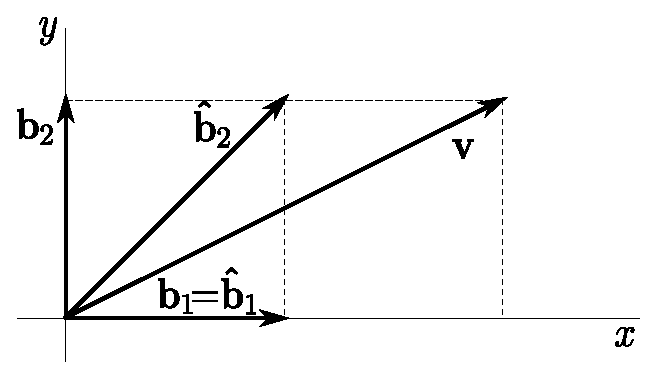
\includegraphics[width=0.90\textwidth]{./fig/ese_basis1.eps}
\end{center}
\end{minipage}
\end{tabular}
%
Il vettore $\bm{v} = 2\bm{b}_1 + 1 \bm{b}_2$ espresso nella base $B_i$ è un dato del problema. Le componenti contravarianti $v^i$ sono $v^1 = 2$, $v^2=1$.
%
Per calcolare la base reciproca $B^i = \left\{ \bm{b}^1 , \bm{b}^2 \right\}$ e le rispettive componenti covarianti con le espressioni (\ref{eqn:b2bd}) e (\ref{eqn:v2vd}) è necessario calcolare i simboli $g_{ik}$ e $g^{ik}$. 
Si calcolano i simboli $g_{ik}$ usando la definizione $g_{ik} = \bm{b}_i \cdot \bm{b}_k$
\begin{equation}
 g_{11} = 1 , \quad g_{12} = g_{21} = 0 , \quad g_{22} = 1
 \quad \Rightarrow \quad
 G = \begin{bmatrix} g_{11} & g_{12} \\ g_{21} & g_{22} \end{bmatrix}
   = \begin{bmatrix} 1 & 0 \\ 0 & 1 \end{bmatrix} ,
\end{equation}
 dove è stata introdotta la matrice $G$ che raccoglie gli elementi $g_{ik}$. I simboli $g^{ik}$ sono gli elementi dell'inversa di $G$, rappresentando la trasformazione inversa $\bm{b}^i = g^{ik}\bm{b}_k$, dagli elementi della base contravariante a quelli della base covariante,
\begin{equation}
 \begin{bmatrix} g^{11} & g^{12} \\ g^{21} & g^{22} \end{bmatrix} = G^{-1} =
 \begin{bmatrix} 1 & 0 \\ 0 & 1 \end{bmatrix} .
\end{equation}
%
Dalla (\ref{eqn:b2bd}) segue che
\begin{equation}
\begin{aligned}
 \bm{b}^1 & = g^{11} \bm{b}_1 + g^{12} \bm{b}_2 = \bm{b}_1 , \\
 \bm{b}^2 & = g^{21} \bm{b}_1 + g^{22} \bm{b}_2 = \bm{b}_2 .
\end{aligned}
\end{equation}
Si poteva ottenere questo risultato senza svolgere nessun conto, poiché la base reciproca di una \textit{base ortonormale}, come $B_i$, coincide con la base stessa. Come conseguenza, anche le componenti covarianti coincidono con le componenti contravarianti,
\begin{equation}
  v_1 = v^1 = 2 , \quad v_2 = v^2 = 1 .
\end{equation}
%
Per calcolare le componenti del vettore $\bm{v}$ nella base $\hat{B}_i$ è necessario calcolare gli elementi della matrice $T$ che esprime il cambiamento di base (\ref{eqn:b2b:t}). \'E possibile ottenere gli elementi di $T$ moltiplicando scalarmente la (\ref{eqn:b2b:t}) per i vettori della base $\bm{\hat{b}}^j$ e sfruttando la definizione di base reciproca (\ref{eqn:def:bd}),
\begin{equation}\label{eqn:eseTrasf}
 \bm{\hat{b}}^j \cdot \bm{b}_k = \bm{\hat{b}}^j \cdot \hat{T}^{q}_{k} \bm{\hat{b}}_{q} = \hat{T}^{j}_{k} .
\end{equation}
%
Per utilizzare la formula precedente è necessario conoscere la base reciproca $\hat{B}^i$. Data la base  Seguendo lo stesso procedimento svolto in precedenza, si calcolano i simboli $\hat{g}_{ik} = \bm{\hat{b}}_i \cdot \bm{\hat{b}}_k$
\begin{equation}
 \hat{g}_{11} = 1 , \quad \hat{g}_{12} = \hat{g}_{21} = 1 , \quad \hat{g}_{22} = 2
\quad \Rightarrow \quad
 \hat{G} = \begin{bmatrix} \hat{g}_{11} & \hat{g}_{12} \\
                           \hat{g}_{21} & \hat{g}_{22} \end{bmatrix}
         = \begin{bmatrix} 1 & 1 \\ 1 & 2 \end{bmatrix}
\end{equation}
 e la trasformazione inversa per ottenere i simboli $\hat{g}^{ik}$,
\begin{equation}
 \begin{bmatrix} \hat{g}^{11} & \hat{g}^{12} \\
                 \hat{g}^{21} & \hat{g}^{22} \end{bmatrix} = \hat{G}^{-1} =
 \begin{bmatrix} 2 & -1 \\ -1 & 1 \end{bmatrix} .
\end{equation}
I vettori dell base controvariante si ottengono dalla (\ref{eqn:b2bd}),
\begin{equation}
\begin{aligned}
 \bm{\hat{b}}^1 & = \hat{g}^{11} \bm{\hat{b}}_1 + \hat{g}^{12} \bm{\hat{b}}_2 = 
      2 \bm{\hat{b}}_1 - \bm{\hat{b}}_2  , \\
 \bm{\hat{b}}^2 & = \hat{g}^{21} \bm{\hat{b}}_1 + \hat{g}^{22} \bm{\hat{b}}_2 =
     - \bm{\hat{b}}_1 + \bm{\hat{b}}_2 .
\end{aligned}
\end{equation}
\'E ora possibile utilizzare la (\ref{eqn:eseTrasf}) per calcolare gli elementi della matrice $\hat{T}$
\begin{equation}
\begin{aligned}
 \hat{T}^{1}_{1} &= \bm{\hat{b}}^1 \cdot \bm{b}_1 = 
  (2 \bm{\hat{b}}_1 - \bm{\hat{b}}_2) \cdot \bm{b}_1 = 
   2 - 1 = 1 ,  \\
 \hat{T}^{1}_{2} &= \bm{\hat{b}}^1 \cdot \bm{b}_2 = 
  (2 \bm{\hat{b}}_1 - \bm{\hat{b}}_2) \cdot \bm{b}_2 = 
   0 - 1 = -1 ,  \\
 \hat{T}^{2}_{1} &= \bm{\hat{b}}^2 \cdot \bm{b}_1 = 
  (- \bm{\hat{b}}_1 + \bm{\hat{b}}_2) \cdot \bm{b}_1 = 
   -1 + 1 = 0 ,  \\
 \hat{T}^{2}_{2} &= \bm{\hat{b}}^2 \cdot \bm{b}_2 = 
  (- \bm{\hat{b}}_1 + \bm{\hat{b}}_2) \cdot \bm{b}_2 = 
    0 + 1 = 1 ,  \\
\end{aligned}
 \quad \Rightarrow \quad
 \hat{T} = \begin{bmatrix} \hat{T}^1_1 & \hat{T}^1_2 \\ \hat{T}^2_1 & \hat{T}^2_2 \end{bmatrix}
   = \begin{bmatrix} 1 & -1 \\ 0 & 1 \end{bmatrix}
\end{equation}
 e la matrice inversa
\begin{equation}
 T = \hat{T} = \begin{bmatrix} T^1_1 & T^1_2 \\ T^2_1 & T^2_2 \end{bmatrix} =
 \begin{bmatrix} 1 & 0 \\ -1 & 1 \end{bmatrix} .
\end{equation}
Utilizzando la (\ref{eqn:v2v:t}) è ora possibile ricavare le componenti del vettore $\bm{v}$ nella base $\hat{B}_i$,
\begin{equation}
\begin{aligned}
 \hat{v}^1 = \hat{T}^1_k v^k = \hat{T}^1_1 v^1 + \hat{T}^1_2 v^2 = 
             1 \cdot 2 - 1 \cdot 1 = 1 \\
 \hat{v}^2 = \hat{T}^2_k v^k = \hat{T}^2_1 v^1 + \hat{T}^2_2 v^2 = 
             0 \cdot 2 + 1 \cdot 1 = 1 \\
\end{aligned}
\quad \Rightarrow \quad 
 \bm{v} = \bm{\hat{b}}_1 + \bm{\hat{b}}_2 .
\end{equation}
Si ricavano infine le componenti covarianti nella base $\hat{B}^i$,
\begin{equation}
\begin{aligned}
 \hat{v}_1 & = \hat{g}_{1k} \hat{v}^k = 
   \hat{g}_{11} \hat{v}^1 + \hat{g}_{12} \hat{v}^2 = 
   1 \cdot 1 + 1 \cdot 1 = 2 \\
 \hat{v}_2 & = \hat{g}_{2k} \hat{v}^k = 
   \hat{g}_{21} \hat{v}^1 + \hat{g}_{22} \hat{v}^2 = 
   1 \cdot 1 + 2 \cdot 1 = 3 
\end{aligned}
\quad \Rightarrow \quad 
 \bm{v} = 2 \bm{\hat{b}}^1 + 3 \bm{\hat{b}}^2 .
\end{equation}
%
%[h!]%[][h!]%[h!]
\begin{figure}
\centering
   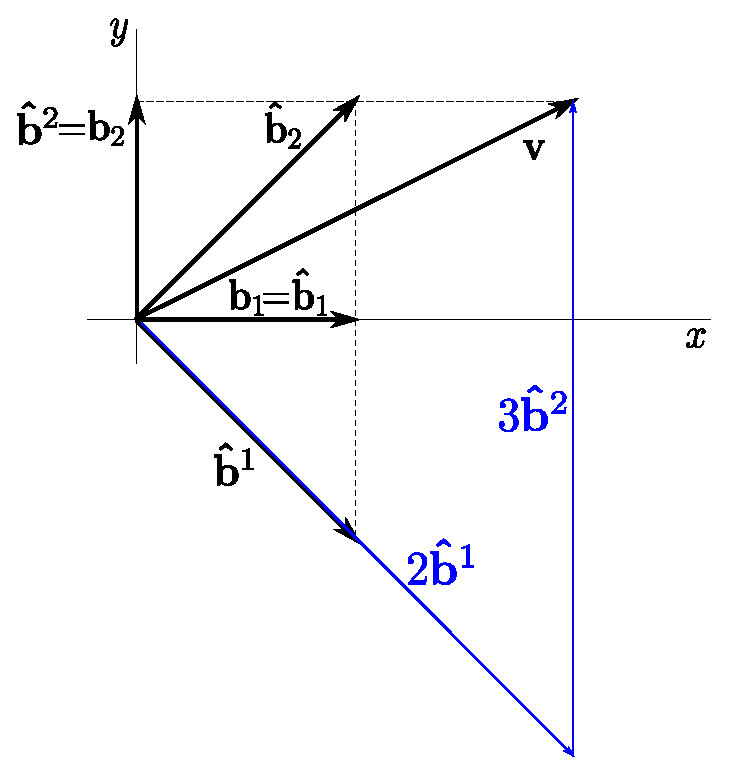
\includegraphics[width=0.60\textwidth]{./fig/ese_basis2.eps}
 \caption{Rappresentazione grafica dell'esempio \ref{exa:basis}.}
\end{figure}
%
Le leggi di trasformazione degli elementi di basi differenti e delle relative componenti sono state introdotte in questo paragrafo per i vettori. Nel prossimo paragrafo verranno utilizzate per ottenere le leggi di trasformazione degli elementi della base e delle componenti dei tensori. In particolare, la definizione classica di tensore come oggetto invariante al cambio di sistema di riferimento, coinvolge direttamente la legge di trasformazione delle componenti, in seguito a un cambio di base. L'esempio \ref{exa:basis} è stato pensato come un'occasione per riprendere dimestichezza con l'analisi lineare e prendere familiarità con le definizione introdotte nel paragrafo.


% ##############################################################
\newpage
% Definizione di secondo spazio duale V**, isomorfismo canonico tra V e V**: conseguenze pratiche ...
%    ...

\section{Algebra multilineare}
Se l'algebra lineare è la branca della matematica che si occupa dello studio dei vettori, degli spazi vettoriali (o spazi lineari) e delle trasformazioni lineari, l'algebra multilineare si occupa dello studio dei tensori, degli spazi tensoriali e delle trasformazioni multilineari.

% Definizione di tensore come funzione multilineare (p,q)
\begin{definition}[Tensore (definizione intrinseca)]\label{def:tensIntrinseca}
 Un tensore di ordine $r$ su $\mathcal{V}$ è una funzione
 $r$-lineare
\begin{equation}
   T : \underbrace{\mathcal{V}   \times \dots \times \mathcal{V}  }_{\text{r volte}} \rightarrow K
%  \qquad \qquad  ( T : \mathcal{V}^r \rightarrow K)
\end{equation}
\end{definition}
%
\begin{remark}
 La definizione di tensore data è riferita agli spazi dotati di prodotto interno. Per una prima introduzione all'algebra e al calcolo tensoriale, può essere considerata un buon compromesso tra comprensibilità e completezza della trattazione, per un corso di ingegneria. Senza voler entrare nei particolari, questa definizione evita di introdurre le definizioni di spazio duale e di isomorfismi necessarie a una trattazione generale dei tensori su spazi vettoriali qualsiasi.
\end{remark}
%
  Si indica con $\mathcal{T}^r(\mathcal{V})$ l'insieme dei tensori di ordine $r$. Questo insieme è chiuso\footnote{Un insieme $\mathcal{V}$ è chiuso rispetto a un'operazione se l'operazione su ogni elemento di $\mathcal{V}$ restituisce un elemento di $\mathcal{V}$.} rispetto alle operazioni di somma e moltiplicazione per uno scalare definite in seguito, e quindi è definito lo spazio vettoriale dei tensori di ordine $r$. %, operazioni rispetto alle quali uno spazio vettoriale deve essere chiuso) 
 Un tensore di ordine $0$ è uno scalare, un tensore di ordine $1$ un vettore.
 
 \subsection{Alcune operazioni tensoriali (I): somma e moltiplicazione per uno scalare.}\label{ch:tensori:operazioniI}
 Le due operazioni di somma e moltiplicazione per uno scalare e la chiusura dell'insieme $\mathcal{T}^r$ rispetto ad esse sono condizioni necessarie alla struttura di spazio vettoriale. La somma di due tensori $\bm{A},\bm{B} \in \mathcal{T}^r(\mathcal{V})$ e la moltiplicazione di $\bm{A}$ per uno scalare $\alpha \in K$ sono definite come
\begin{equation}\label{eqn:tens:somma}
 (\bm{A}+\bm{B})(\bm{u}^1,\dots,\bm{u}^r) = 
   \bm{A} (\bm{u}^1,\dots,\bm{u}^r) +
   \bm{B} (\bm{u}^1,\dots,\bm{u}^r)
\end{equation}
 e
\begin{equation}\label{eqn:tens:moltScal}
 ( \alpha \bm{A} ) (\bm{u}^1,\dots,\bm{u}^r) = 
   \alpha \bm{A}   (\bm{u}^1,\dots,\bm{u}^r)
\end{equation}
 per ogni $r$-upla di vettori $(\bm{u}^1,\dots,\bm{u}^r) \in \mathcal{V}^r$.
%
\vspace{15pt}
\begin{definition}[Spazio vettoriale $\mathcal{T}^r(\mathcal{V})$ dei tensori di ordine $r$] Lo spazio vettoriale $\mathcal{T}^r(\mathcal{V})$ dei tensori di ordine $r$ sullo spazio $\mathcal{V}$ è formato dall'insieme $\mathcal{T}^r(\mathcal{V})$, con le operazioni di somma e moltiplicazione per uno scalare definite in (\ref{eqn:tens:somma}) e (\ref{eqn:tens:moltScal}).
\end{definition}
%
 \subsection{Prodotto tensoriale} Dati r vettori $\bm{v}_1,\dots,\bm{v}_r \in \mathcal{V}$  si definisce il prodotto tensoriale tra vettori
 $\bm{v}_1 \otimes \dots \otimes \bm{v}_r$ come
\begin{equation}
  \bm{v}_1 \otimes \dots \otimes \bm{v}_r 
  (\bm{u}^1,\dots,\bm{u}^r) = 
  (\bm{v}_1 \cdot \bm{u}^1) \dots ( \bm{v}_r \cdot \bm{u}^r ) ,
\end{equation}
 per ogni $r$-upla di vettori $(\bm{u}^1,\dots,\bm{u}^r) \in \mathcal{V}^r$.
 
 \noindent
 Per due tensori $\bm{A} \in \mathcal{T}^p(\mathcal{V})$, $\bm{B} \in \mathcal{T}^r(\mathcal{V})$
 il prodotto $\bm{A} \otimes \bm{B} \in \mathcal{T}^{p+r}(\mathcal{V})$ è definito come
\begin{equation}
 (\bm{A}\otimes\bm{B})(\bm{u}^1,\dots,\bm{u}^{p+r}) = 
   \bm{A} (\bm{u}^1,\dots,\bm{u}^p)
   \bm{B} (\bm{u}^{p+1},\dots,\bm{u}^{p+r}) ,
\end{equation}
 per ogni $(\bm{u}^1,\dots,\bm{u}^{p+r}) \in \mathcal{V}^{p+r}$.

 \noindent
 \begin{remark}
 Il prodotto tensoriale \textbf{non} è commutativo: $\bm{A} \otimes \bm{B} \neq \bm{B} \otimes \bm{A}$.
 \end{remark}

%  \section{Spazio dei tensori di ordine r $\mathcal{T}^r(\mathcal{V})$}
% L'insieme dei tensori di ordine $r$ costituisce uno spazio vettoriale, indicato con $\mathcal{T}^r(\mathcal{V})$,
% una volta definite le operazioni chiuse di somma e di moltiplicazione per uno scalare.
 
\begin{definition}[Base prodotto di $\mathcal{T}^r(\mathcal{V})$] Se lo spazio $\mathcal{V}$
 ha dimensione $N$, la dimensione dello spazio $\mathcal{T}^r(\mathcal{V})$ è $N^r$.
 La base $\{ \bm{b}_k \}_{k=1:N}$ di $\mathcal{V}$
 induce una base prodotto (covariante) di $\mathcal{T}^r(\mathcal{V})$, definita come
\begin{equation}
  \left\{ \bm{b}_{i_1} \otimes \dots \otimes \bm{b}_{i_r} \right\}_{
  i_1,\dots,i_r = 1 : N} .
\end{equation}
\end{definition}
%
\noindent
 Rispetto alla base prodotto, un tensore $\bm{A} \in \mathcal{T}^r(\mathcal{V})$ viene scritto come
 \begin{equation}
  \bm{A} = A^{i_1 \dots i_r} \bm{b}_{i_1} \otimes \dots \otimes \bm{b}_{i_r} ,
 \end{equation}
 dove $A^{i_1 \dots i_r}$ sono le componenti contravarianti del tensore $\bm{A}$ rispetto alla base prodotto covariante.
 Si dimostra che le componenti $A^{i_1 \dots i_r}$ sono
 \begin{equation}
   A^{i_1 \dots i_r} = \bm{A}(\bm{b}^{i_1},\dots,\bm{b}^{i_r}) .
 \end{equation}
 Infatti,
 \begin{equation}
 \begin{aligned}
   \bm{A}(\bm{b}^{k_1},\dots,\bm{b}^{k_r}) & =
     A^{i_1 \dots i_r} \bm{b}_{i_1} \otimes \dots \otimes \bm{b}_{i_r} ( \bm{b}^{k_1}, \dots, \bm{b}_{l_r})  = \\ & =
     A^{i_1 \dots i_r} ( \bm{b}_{i_1} \cdot \bm{b}^{k_1} ) \dots (\bm{b}_{l_r} \cdot \bm{b}^{j_r} )  = \\
     & = A^{i_1 \dots i_r} \delta^{k_1}_{i_1} \dots \delta^{j_r}_{l_r} = A^{k_1 \dots k_r}
 \end{aligned}
 \end{equation}

%  le componenti di un tensore $\bm{A} \in \mathcal{T}^p_q(\mathcal{V})$ sono $N^(p+q)$ scalari 
% definiti come
%\begin{equation}
%  A^{i_1 \dots i_p}_{\ \ \ j_1 \dots j_q} = \bm{A}(\bm{b}^{i_1},\dots,\bm{b}^{i_p},\bm{b}_{j_1},\dots,\bm{b}_{j_q})
%\end{equation}
% e il tensore $\bm{A}$ può esere scritto in componenti come
%\begin{equation}
%  \bm{A} = A^{i_1 \dots i_p}_{\ \ \ j_1 \dots j_q} \bm{b}_{i_1} \otimes \dots \otimes \bm{b}_{i_p} \otimes
%   \bm{b}^{j_1} \otimes \dots \otimes \bm{b}^{j_q}
%\end{equation}
 
 \subsection{Trasformazione tra oggetti controvarianti e covarianti: regola per ``alzare e abbassare gli indici''.}
 Nei paragrafi precedenti è stata ricavata la regola per ricavare le componenti contravarianti di un vettore dalle compontenti
 covarianti e viceversa. In questo paragrafo verranno ricavate le regole per alzare e abbassare gli indici in un tensore di 
 ordine $r$ generico, seguendo un procedimento simile a quello seguito in precedenza.
 Come primo esempio, si parte da un tensore scritto nella base prodotto covariante, con indici bassi
 (quindi le coomponenti hanno tutti indici contravarianti, alti): l'obiettivo è quello di scrivere le componenti in una base con il primo vettore
 appartenente alla base reciproca (indice alto) e tutti gli altri uguali (indici bassi). Le componenti avranno quindi il primo
 indice basso e gli altri alti.
 \begin{equation}
 \begin{aligned}
  \bm{A} & = A^{i_1 \dots i_r} \bm{b}_{i_1} \otimes \bm{b}_{i_2} \otimes \dots \otimes \bm{b}_{i_r} = \\
         & = A^{i_1 \dots i_r} g_{i_1 k_1} \bm{b}^{k_1} \otimes \bm{b}_{i_2} \otimes \dots \otimes \bm{b}_{i_r} = \\
         & = g_{i_1 k_1}A^{k_1 \dots i_r} \bm{b}^{i_1} \otimes \bm{b}_{i_2} \otimes \dots \otimes \bm{b}_{i_r} = \\
         & = A_{i_1}^{\ i_2 \dots i_r} \bm{b}^{i_1} \otimes \bm{b}_{i_2} \otimes \dots \otimes \bm{b}_{i_r}
 \end{aligned}
 \end{equation}
 dove è stata usata la simmetria dei simboli $g_{ij} = g_{ji}$ e sono stati invertiti gli indici ripetuti (sono indici ``dummy'',
 saturati dalla sommatoria). Risulta quindi
 \begin{equation}\label{eqn:t2td}
   A_{i_1}^{\ \ i_2\dots i_r} = g_{i_1 k_1} A^{k_1 i_2 \dots i_r}
 \end{equation}
 dove come sempre è sottointesa la sommatoria sugli indici ripetuti (qui solo $k_1$). Una volta capito il ruolo di $g_{ij}$ nell'abbassamento
 e nell'innalzamento degli indici, la stessa regola può essere applicata a qualsiasi indice di un tensore di ordine qualsiasi.

% 
 \subsection{Cambio di base e regola di trasformazione delle componenti: definizione ``classica'' di tensore.} 
%
 Aiutandosi con la legge di trasformazione degli elementi della base $\{ \bm{b}_k \}_{k=1:N}$ di $\mathcal{V}$ 
 e della base reciproca $\{ \bm{b}^k \}_{k=1:N}$ di $\mathcal{V}^*$, si può verificare
  che la base prodotto (covariante) dello spazio $\mathcal{T}^r(\mathcal{V})$ si trasforma secondo
\begin{fBox}
\begin{equation}\label{eqn:bp2bp:t}
\begin{aligned}
 &  \bm{\hat{b}}_{i_1} \otimes \dots \otimes \bm{\hat{b}}_{i_r} = 
  T^{k_1}_{i_1}\dots T^{k_p}_{i_r}
  \bm{b}_{k_1} \otimes \dots \otimes \bm{b}_{k_r} \\
  &  \bm{b}_{i_1} \otimes \dots \otimes \bm{b}_{i_r} = 
  \hat{T}^{k_1}_{i_1}\dots \hat{T}^{k_r}_{i_r}
  \bm{\hat{b}}_{k_1} \otimes \dots \otimes \bm{\hat{b}}_{k_r} .
\end{aligned}
\end{equation}
\end{fBox}
 Per ricavare la regola di trasformazione della base prodotto (\ref{eqn:bp2bp:t}) è sufficiente applicare la (\ref{eqn:b2b:t}) a tutti i vettori $\bm{b}_{i_\alpha}$ della base prodotto.  Usando la multilinearità del prodotto tensoriale
 \begin{equation}
 \begin{aligned}
  \bm{\hat{b}}_{i_1} \otimes \dots \otimes \bm{\hat{b}}_{i_r} = &
  ( T^{k_1}_{i_1}\bm{b}_{k_1} ) \otimes \dots \otimes ( T^{k_p}_{i_r}\bm{b}_{k_r}) = \\
  = & T^{k_1}_{i_1}\dots T^{k_r}_{i_r}
   \bm{b}_{k_1} \otimes \dots \otimes \bm{b}_{k_r} . \\
 \end{aligned}
 \end{equation}
%
 La regola di trasformazione delle componenti di un tensore $\bm{A} \in \mathcal{T}^r(\mathcal{V})$, $\bm{A} =$ $A^{i_1 \dots i_r} \bm{b}_{i_1} \otimes \dots \otimes \bm{b}_{i_r} =$ $\hat{A}^{i_1 \dots i_r} \bm{\hat{b}}_{i_1} \otimes \dots \otimes \bm{\hat{b}}_{i_r} $ al variare dei sistemi di riferimento è
\begin{fBox}
\begin{equation}\label{eqn:t2t:t}
\begin{aligned}
 &  \hat{A}^{k_1 \dots k_r} = 
  \hat{T}^{k_1}_{i_1}\dots \hat{T}^{k_r}_{i_r} A^{i_1 \dots i_r} \\
 &  A^{i_1 \dots i_r} = 
  T^{i_1}_{k_1}\dots T^{i_r}_{k_r} 
  \hat{A}^{k_1 \dots k_r} .
\end{aligned}
\end{equation}
\end{fBox}
 %
 La legge di trasformazione delle componenti (\ref{eqn:t2t:t}) si ricava grazie alla legge di trasformazione della base prodotto
 \begin{equation}
 \begin{aligned}
  \bm{A} & =  A^{i_1 \dots i_r} \bm{b}_{i_1} \otimes \dots \otimes \bm{b}_{i_r} = \\
   & = A^{i_1 \dots i_r}
     \hat{T}^{k_1}_{i_1}\dots \hat{T}^{k_r}_{i_r} 
     \bm{\hat{b}}_{k_1} \otimes \dots \otimes \bm{\hat{b}}_{k_r} = \\ 
   & = \hat{A}^{k_1 \dots k_r} \bm{\hat{b}}_{k_1} \otimes \dots \otimes \bm{\hat{b}}_{k_r}
 \end{aligned}
 \end{equation}
%
Partendo dalla definizione intrinseca di un tensore come applicazione multilineare \ref{def:tensIntrinseca}, grazie all'introduzione di una base dello spazio vettoriale e alla rappresentazione in coordinate, è stato possibile arrivare alla definizione classica di tensore.
\vspace{15pt}
\begin{definition}[Tensore (definizione classica)]
Un tensore $\bm{A}$ di ordine $r$ su uno spazio $\mathcal{V}$ di dimensione $N$ è un oggetto matematico formato da $N^r$ componenti $A^{i_1 \dots i_r}$ che si trasformano secondo la (\ref{eqn:t2t:t}), in seguito al cambio di sistema di coordinate $\bm{b}_j = \hat{T}^i_j \bm{\hat{b}}_i$.
\end{definition}

%
 \subsection{Alcune operazioni tensoriali (II)}\label{ch:tensori:operazioniII}
%
 Come le operazioni introdotte nel paragrafo \ref{ch:tensori:operazioniI}, anche le operazioni in questo paragrafo operano su tensori e restituiscono tensori.
 
 \subsubsection{Contrazione.} L'operazione di contrazione $\bm{C}^k_l$ agente su un tensore $\bm{A}$ di ordine $r$ ha come risultato un tensore di ordine $r-2$. Le componenti del tensore ottenuto tramite la contrazione di due indici si ottengono saturando con la somma gli indici di tutte le componenti indicati da $\bm{C}^k_l$
\begin{equation}\label{eqn:defContrazione}
\begin{aligned}
 \bm{C}^k_l \bm{A} & =
 \bm{C}^k_l \big(A^{i_1 \dots i_r} \bm{b}_{i_1} \otimes \dots \otimes \bm{b}_{i_r}\big) \\
 & = \bm{C}^k_l \big(A^{i_1 \dots i_k \dots i_{l-1} \ i_{l+1} \dots i_r}_{\qquad \quad \ i_l} \bm{b}_{i_1} \otimes \dots \otimes \bm{b}_{i_k} \otimes \dots \otimes \bm{b}_{i_{l-1}} \otimes  \bm{b}^{i_l} \otimes \bm{b}_{i_{l+1}} \otimes \dots \otimes \bm{b}_{i_r}\big) \\
 & = A^{i_1 \dots i_{k-1} n i_{k+1} \dots i_{l-1} \ i_{l+1} \dots i_r}_{\qquad \qquad \quad \ \ n} \bm{b}_{i_1} \otimes \dots \otimes \bm{b}_{i_{k-1}} \otimes \bm{b}_{i_{k+1}} \otimes \dots \otimes \bm{b}_{i_{l-1}} \otimes \bm{b}_{i_{l+1}} \otimes \dots \otimes \bm{b}_{i_r} .
\end{aligned}
\end{equation}
Per rendere (più) comprensibile la definizione dell'operazione di contrazione data in (\ref{eqn:defContrazione}), si fornisce un esempio su un tensore di ordine 3, $\bm{A} = A^{ijk} \bm{b}_i \otimes \bm{b}_j \otimes \bm{b}_k$.
\begin{remark}
 Affinchè la contrazione sia svolta correttamente (e quindi dia come risultato un tensore) senza la scrittura esplicita dei simboli $g_{ik}$, la coppia di indici che viene ``contratta'' deve avere carattere opposto (uno covariante, l'altro contravariante).
\end{remark}
  Si vuole svolgere la contrazione del primo e del terzo indice di $\bm{A}$. In componenti si ottiene
  \begin{equation}
   \bm{C}^1_3 \bm{A} = \bm{C}^1_3 ( A^{ijk} \bm{b}_i \otimes \bm{b}_j \otimes \bm{b}_k ) =  \bm{C}^1_3 ( A_i^{\ \ jk} \bm{b}^i \otimes \bm{b}_j \otimes \bm{b}_k ) = A_i^{\ \ ji} \bm{b}_j = g_{il} A^{ljk} \bm{b}_j ,
  \end{equation}
  dove è stata utilizzata la regola (\ref{eqn:t2td}) per esprimere il risultato in funzione del tensore $\bm{A}$ con tutti gli indici contravarianti.
% $A_i^{\ jk} = g_{il} A^{ljk}$. Quindi $A_i^{\ \ ji} = g_{il} A^{lji}$, dove sono sottointese le somme sugli indici $i$, $l$.
  
 \subsubsection{``Dot'' product.} Siano $\bm{A} \in \mathcal{T}^r(\mathcal{V})$, $\bm{B} \in \mathcal{T}^s(\mathcal{V})$, il
 prodotto ``dot'' $\bm{A} \cdot \bm{B}$ è un tensore di ordine $r+s-2$, definito tramite il prodotto tensoriale e la contrazione
 di una coppia di indici di natura opposta.
 In particolare si definisce 
 \begin{equation}
  \bm{A} \cdot \bm{B} = \bm{C}^{r}_{r+1} (\bm{A} \otimes \bm{B}) .
 \end{equation}
 Si ricorda che la contrazione deve avvenire tra indici di natura opposta. Supponendo che la regola per passare da indici
 covarianti a indici contravarianti sia stata compresa e non comporti nessuna difficoltà aggiuntiva, per comodità il tensore
 $\bm{A}$ viene scritto in componenti contravarianti, il tensore $\bm{B}$ in componenti covarianti. Facendo un esempio con
 $\bm{A} \in \mathcal{T}^3$, $\bm{B} \in \mathcal{T}^2$
 \begin{equation}
 \begin{aligned}
  \bm{A} \cdot \bm{B} & = (A^{ijk} \bm{b}_i \otimes \bm{b}_j \otimes \bm{b}_k) \cdot (B_{mn} \bm{b}^m \otimes \bm{b}^n) = \\
   & = A^{ijk} B_{mn} \bm{b}_i \otimes \bm{b}_j \otimes \bm{b}_k \cdot \bm{b}^m \otimes \bm{b}^n = \\
   & = A^{ijl} B_{ln} \bm{b}_i \otimes \bm{b}_j \otimes \bm{b}^n .
 \end{aligned}
 \end{equation}
%
\begin{remark}
 Il prodotto ``dot'' \textbf{non} è commutativo ($\bm{A} \cdot \bm{B} \neq \bm{B} \cdot \bm{A}$).
 Il prodotto ``dot'' \textbf{non} è un prodotto interno (in generale non ha nemmeno come risultato uno scalare).
\end{remark}
 
 \subsubsection{Doppio ``Dot'' product.}
 Siano $\bm{A} \in \mathcal{T}^r(\mathcal{V})$, $\bm{B} \in \mathcal{T}^s(\mathcal{V})$, il doppio prodotto ``dot'' $\bm{A} : \bm{B}$ è un tensore di ordine $r+s-4$ definito tramite il prodotto tensoriale e una doppia contrazione.
  In particolare si definisce
 \begin{equation}
  \bm{A} : \bm{B} = \bm{C}^{r-1,r}_{r+1,r+2} (\bm{A} \otimes \bm{B})
 \end{equation}
 Per esempio con $\bm{A} \in \mathcal{T}^4$, $\bm{B} \in \mathcal{T}^3$:
 \begin{equation}
 \begin{aligned}
  \bm{A} : \bm{B} & = (A^{ijkl} \bm{b}_i \otimes \bm{b}_j \otimes \bm{b}_k\otimes \bm{b}_l)
                             : (B_{mnp} \bm{b}^m \otimes \bm{b}^n \otimes \bm{b}^p) = \\
   & = A^{ijuv} B_{uvp} \bm{b}_i \otimes \bm{b}_j  \otimes \bm{b}^p
 \end{aligned}
 \end{equation}
 Si presti attenzione all'ordine con il quale avviene la doppia contrazione: il penultimo indice di $\bm{A}$ si contrae con il primo di $\bm{B}$, l'ultimo di $\bm{A}$ con il secondo di $\bm{B}$. \'E possibile definire ``dot product'' multipli estendendo la contrazione a un numero maggiore di indici.
 
\begin{example}[Tensore degli sforzi]
 I primi tensori che vengono incontrati durante un corso di studi in ingegneria sono il tensore di inerzia per i corpi rigidi in Meccanica Razionale e il tensore degli sforzi nei corsi di Meccanica Strutturale.  
Viene qui ricavato velocemente il legame tra vettore sforzo $\bm{t_n}$ e la normale $\bh{n}$ della giacitura considerata in un mezzo continuo non polare, tramite l'equilibrio del tetraedro di Cauchy. Siano $\bh{x}$, $\bh{y}$ e $\bh{z}$ i versori di un sistema di riferimento cartesiano centrato nel punto del continuo considerato e $\bh{e}_{\bm{x}} = \bm{t_x}$, $\bh{e}_{\bm{y}} = \bm{t_y}$ e $\bh{e}_{\bm{z}} = \bm{t_z}$ i vettori sforzo agenti sulle facce del tetraedro di area $dS_x$, $dS_y$ e $dS_z$ con le normali orientate come i rispettivi versori della base. Sia $\bm{t_n}$ il vettore sforzo agente sulla faccia ``inclinata'' di area $dS$ del tetraedro di Cauchy, con normale $\bh{n}$. Il legame tra le aree delle facce del tetraedro è
\begin{equation}
 dS = - \dfrac{dS_x}{n_x} = - \dfrac{dS_y}{n_y} = - \dfrac{dS_z}{n_z} ,
\end{equation}
avendo indicato con $n_i$ le componenti cartesiane del versore normale $\bh{n}$, tutte negative per come è stato definito il tetraedro rappresentato in figura \ref{fig:tetraedroCauchy}. Si scrive l'equilibrio del tetraedro, ricordando che i contributi di volume sono di un ordine inferiore rispetto a quelli di superficie, quando le dimensioni del tetraedro tendono a zero,
\begin{equation}
\begin{aligned}
 \bm{0} & = \bm{t_n} dS + \bm{t_x} dS_x + \bm{t_y} dS_y + \bm{t_z} dS_z = \\
  & = ( \bm{t_n} - \bm{t_x} n_x - \bm{t_y} n_y - \bm{t_z} n_z ) dS  \qquad \rightarrow \qquad \bm{t_n} = \bm{t_x} n_x + \bm{t_y} n_y + \bm{t_z} n_z \\
\end{aligned}
\end{equation}
Secondo la definizione intrinseca, il vettore $\bm{t_n}$ è un'applicazione lineare $\bm{t_n}: \mathcal{V} \rightarrow K = \mathbb{R}$, la cui azione su un vettore qualsiasi $\bm{v} \in \mathcal{V}$ può essere espressa in termini del prodotto scalare su $\mathcal{V}$,
\begin{equation}
\begin{aligned}
\bm{t_n}(\bm{v}) = \bm{t_n} \cdot \bm{v} & = \bm{t_x}\cdot \bm{v} n_x + \bm{t_y}\cdot \bm{v} n_y + \bm{t_z}\cdot \bm{v} n_z = \\
& = (\bm{t_x}\cdot \bm{v}) (\bh{x} \cdot \bh{n}) +
    (\bm{t_y}\cdot \bm{v}) (\bh{y} \cdot \bh{n}) +
    (\bm{t_z}\cdot \bm{v}) (\bh{z} \cdot \bh{n}) = (\bh{e}_{\bm{i}} \cdot \bh{n}) (\bm{t_i}\cdot \bm{v}) = \\
& = \left[\bh{e}_{\bm{i}} \ot \bm{t_i}\right] (\bh{n},\bm{v}) = 
 \left[t_{i,j} \bh{e}_{\bm{i}} \ot \bh{e}_{\bm{j}} \right] (\bh{n},\bm{v}) = \bm{T} (\bh{n},\bm{v}) ,
\end{aligned}
\end{equation}
avendo definito $t_{i,j}$ la $j$-esima coordinata del vettore agente sulla $i$-esima faccia e introdotto la defintizione del tensore degli sforzi $\bm{T}$. \'E sottintesa la sommatoria sugli indici ripetuti. Sfruttando l'uguaglianza appena ricavata,  valida per ogni vettore $\bm{v} \in \mathcal{V}$,
\begin{equation}
\begin{aligned}
  \bm{t_n} \cdot \bm{v} & = (\bh{n} \cdot \bh{e}_{\bm{i}}) (\bm{t_i}\cdot \bm{v})
   = \bh{n} \cdot \bh{e}_{\bm{i}} \ot \bm{t_i} \cdot \bm{v} = \\
 & = \bh{n} \cdot \left[t_{i,j} \bh{e}_{\bm{i}} \ot \bh{e}_{\bm{j}} \right] \cdot \bm{v}
   = \bh{n} \cdot \left[T_{ij} \bh{e}_{\bm{i}} \ot \bh{e}_{\bm{j}} \right] \cdot \bm{v}
   = \bh{n} \cdot \bm{T} \cdot \bm{v} ,
\end{aligned}
\end{equation}
 dove sono state definite le componenti $T_{ij} = t_{i,j}$ del tensore degli sforzi in una base cartesiana, si ricava la relazione tra il vettore sforzo $\bm{t_n}$ e la normale $\bh{n}$,
 \begin{equation}\label{eqn:tensor:stressTensor}
  \bm{t_n} = \bh{n} \cdot \bm{T} .
 \end{equation}
\end{example}

\begin{figure}
\centering
 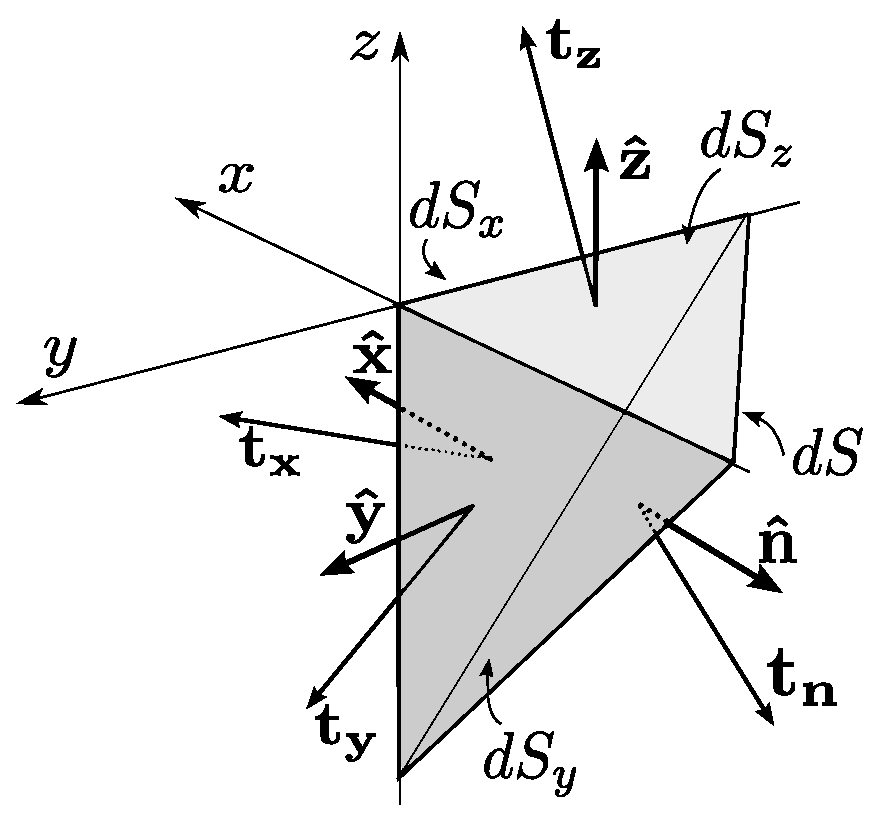
\includegraphics[width=0.60\textwidth]{./fig/cauchy.eps}
\caption{tetraedro di Cauchy}\label{fig:tetraedroCauchy}
\end{figure}

\subsection{Cosa non è stato detto}
 Molte cose non sono state dette. In particolare, è stato scelto di trattare i tensori su spazi forniti di prodotto interno e di non introdurre concetti di \textit{algebra esterna}, che permetterebbero di generalizzare l'operazione di rotore e ricavare il teorema di Stokes,
\begin{equation}
 \oint_{\partial \Omega} \omega = \int_\Omega d\omega ,
\end{equation}
 di cui viene solo riportata l'espressione matematica senza fornire alcun dettaglio. Il teorema del rotore e della divergenza sono casi particolari del teorema di Stokes, nel cui enunciato compaiono i concetti di forma differenziale $\omega$ e di derivata esterna $d \omega$.

 \noindent
Il materiale fornito rappresenta un compromesso tra il vuoto totale sul calcolo tensoriale (del quale l'affermazione ``un tensore è una matrice'' è la regina indiscussa) e un corso intero dedicato al calcolo tensoriale. Lo scopo dei cenni veloci ad argomenti non trattati qui è quello di ``mettere una pulce nell'orecchio'' di chi legge, di mettere a conoscenza il lettore dell'esistenza di alcuni argomenti che permettono di generalizzare le operazioni vettoriali presentate nei primi corsi di Algebra e di spiegare in maniera rigorosa alcuni comportamenti strani o inaspettati (come quelli che si possono osservare con il prodotto vettoriale e il rotore), senza scoperchiare dei vasi di Pandora che porterebbero questa introduzione lontana dal suo scopo.

\vspace{10pt}
 \noindent
 Per i più curiosi, viene messo a disposizione del materiale un più completo, che introduce concetti che non sono stati presentati qui e che generalizzano la trattazione, ma che la renderebbero inadatta ad essere svolta in poche ore per un pubblico formato da studenti del terzo anno di ingegneria, senza aggiungere particolari fondamentali per un utilizzo ``cosciente'' dei tensori durante questo corso e in quelli successivi.

 \subsubsection{Riferimenti.}  
 Il testo di Bowen e Wang, \textit{Introduction to vectors and tensors. Linear and multilinear algebra} può essere considerato un valido e completo riferimento, anche per il futuro. La lettura di questo testo non è sempre agevole e contiene sicuramente molto più di quanto sia indispensabile presentare in una prima e breve introduzione ai tensori, come è questa.
 Oltre alla sua qualità, è da apprezzare la disponibilità in rete dei due volumi, seguendo i seguenti collegamenti (sperando che siano ancora validi):
 
 \href{http://oaktrust.library.tamu.edu/bitstream/handle/1969.1/2502/IntroductionToVectorsAndTensorsVol1.pdf}
 {Vol. 1: Linear and Multilinear Algebra}
 
 \href{http://oaktrust.library.tamu.edu/bitstream/handle/1969.1/3609/IntroductionToVectorsAndTensorsVol2.pdf}
 {Vol. 2: Vector and Tensor Analysis}
 
% http://www.mat.unimi.it/users/carati/didattica/dispense/tensori.pdf
 
 
 \subsubsection{Cosa è utile ripassare.} Questa può essere una buona occasione per ripassare alcuni concetti di algebra lineare, tra i quali quello di spazio vettoriale (definizione e proprietà, dimensione e base, \dots), prodotto interno, linearità (e la differenza con l'essere ``affine''), alla luce di quanto visto in questi paragrafi introduttivi sui tensori e del fatto che le equazioni della fisica hanno carattere tensoriale.




